\section{Results}

A supplied schema improves Nano's notes. Note-format similarity increases within long chains, but does not establish conventions. Same-day tests confirm higher scores with retained reasoning for both Luna models. Tighter budgets reduce frontier scores without establishing a ranking. Detailed cell means and paired tests are grouped in \Cref{app:comparisons}; format diagnostics are in \Cref{app:format}.

\subsection{Supplied structure improves Nano's notes}\label{sec:extern}\label{sec:ladder}
Nano's free-form notes lose accuracy as the budget tightens (\Cref{fig:knee}). At $B{=}100$, they score $\relayextmeanhundred$, compared with $\relayextfullmean$ for the visible transcript: a paired loss of $\relayextlosshundred$ (95\% $t$ CI $[\relayextlosslohundred,\relayextlosshihundred]$; exact sign $p{=}\relayextphundred$; $n{=}\relayextnhundred$). At $B{=}800$, notes average only about \relayextfillmean{} characters. The remaining loss is $\relayextlosseighthundred$ and is unconfirmed ($p{=}\relayextpeighthundred$).

\begin{figure}[htbp]
\centering
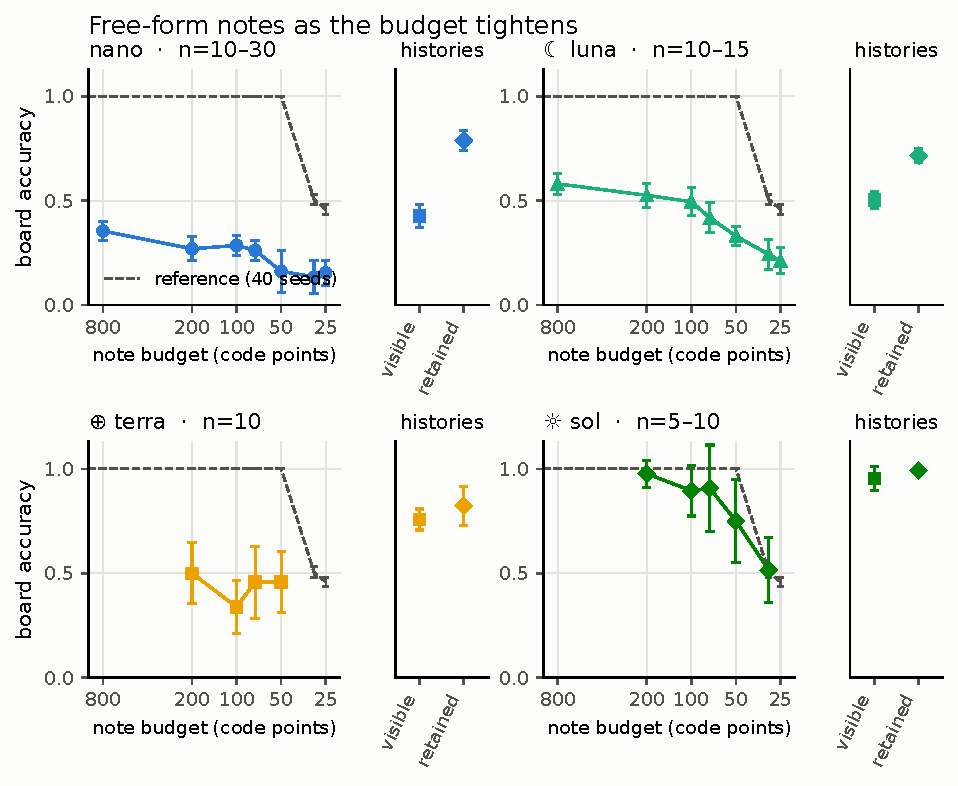
\includegraphics[width=\linewidth]{figures/relay_fig1_knee.pdf}
\caption{Mean board accuracy (fraction of keys correct) with free-form notes and transcript controls for the four original models. Intervals are across-seed 95\% $t$ intervals; cells use all available seeds ($n{=}5$--30; exact counts in \Cref{app:cells}). Numeric budgets follow a descending log axis. Visible and retained histories are separate categorical controls, unconnected to the note-budget curves. Dashed lines show the versioned 40-seed reference mean. These descriptive means do not identify a retention mechanism; the original-model controls span collection dates.}
\label{fig:knee}
\end{figure}

The supplied schema improves Nano's notes by $+\relayprimnanoschematwohundreddelta$ at $B{=}200$ and $+\relayprimnanoschemafiftydelta$ at $B{=}50$. Both survive Holm correction over the declared \relayprimfamily-test family (adjusted $p\relayprimnanoschematwohundredholm$ and $p\relayprimnanoschemafiftyholm$). The $B{=}100$ estimate, $+\relayprimnanoschemahundreddelta$, does not survive correction (adjusted $p\relayprimnanoschemahundredholm$). The harness form also improves scores at $B{=}200$ (adjusted $p\relayprimnanoformtwohundredholm$). These are effects of the supplied interface packages; their role in the model's reasoning is unobserved.

On the separately declared 30-seed comparison at $B{=}100$, schema notes outperform Nano's visible transcript by $+\relayfamtwodelta$ (95\% $t$ CI $[\relayfamtwolo,\relayfamtwohi]$; F2, $p\relayfamtwoholm$). The schema also improves on free-form notes and the visible transcript on the 39-key board (F3). Gemini 3.5 Flash's schema-minus-free-form gain and free-form-minus-visible loss are both unconfirmed after correction (F4; \Cref{tab:families}).

Nano's later retained-reasoning control scores $\relayfamfivestdabs$ above its schema notes (F5; Holm $p\relayfamfivestdholm$) and $\relayfamsevenabs$ above its free-form notes (F7; $p\relayfamsevenp$). These comparisons span collection dates and include any change in the served model. No negative scaffold contrast for the other original models survives family-wise correction (\Cref{tab:contrasts,app:crossover}).

\FloatBarrier

\subsection{Note formats become more similar within long chains}\label{sec:convention}
Luna's notes change notation while remaining compact: \texttt{LMb=A} $\to$ \texttt{Ppt=O} $\to$ \texttt{Lringhome}. We measure this \textbf{notation drift} by comparing consecutive notes after normalizing letters and digits. Similarity then reflects format, length and belief-state shape rather than symbol identity. \Cref{app:format} gives the estimator checks and a complete transmitted sequence.

In Luna's 60-turn-cap runs, mean similarity at successor-note turns 13 onward exceeds similarity at turns 2--7 by $+\relaydriftcleantrendhundred$ at $B{=}100$ (95\% $t$ CI $[\relaydriftcleantrendhundredlo,\relaydriftcleantrendhundredhi]$) and $+\relaydriftcleantrendtwohundred$ at $B{=}200$ ($[\relaydriftcleantrendtwohundredlo,\relaydriftcleantrendtwohundredhi]$). All ten episodes at each budget have a positive difference. This analysis excludes terminal notes, disables the matcher's frequent-character heuristic and averages within episodes before calculating uncertainty.

The within-chain increase survives those checks, but early and late turns also differ in acquired state and rotation exposure. The between-chain metric fails its fixed-codec negative control: reference chains using one notation still become less similar to one another. The evidence therefore supports a surface-format trend, without establishing chain-specific conventions.
\subsection{Retained reasoning improves both Luna controls}\label{sec:retention}
The original four models' retained and visible controls were collected two months apart. Nano's historical retained-minus-visible difference is $+\relayfamsixnanodelta$ (F6; Holm $p\relayfamsixnanoholm$). Luna's estimate is positive but does not survive correction; Terra's and Sol's differences are also unconfirmed (\Cref{tab:families}). These comparisons motivated fresh-seed tests with both controls collected on the same day.

\begin{figure}[htbp]
\centering
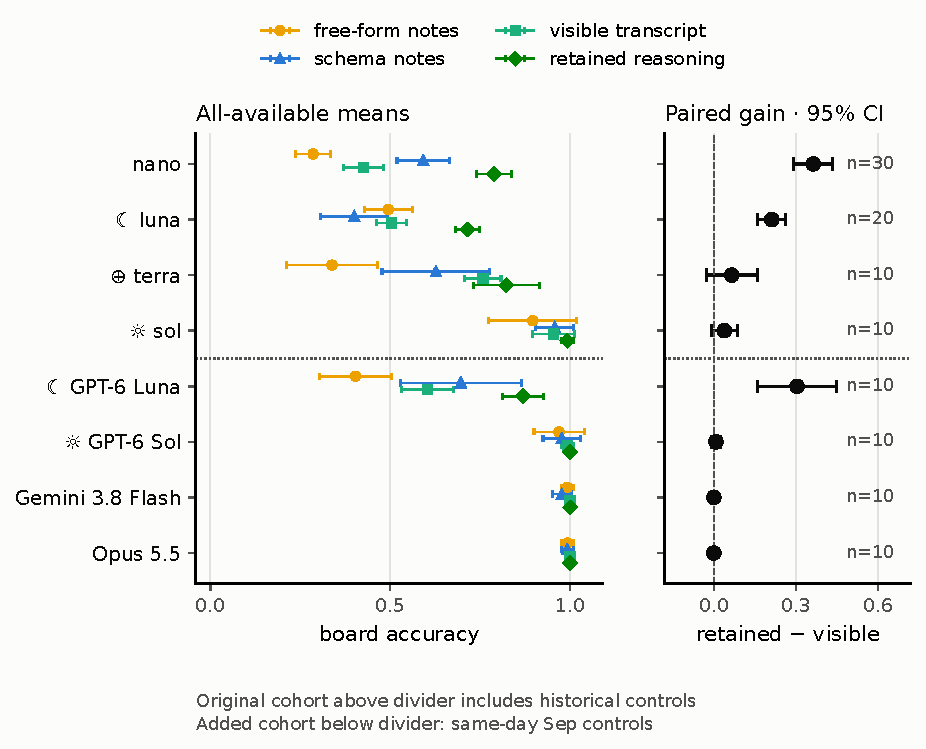
\includegraphics[width=\linewidth]{figures/relay_fig4_models.pdf}
\caption{Board accuracy (fraction of keys correct) across four memory conditions: free-form and schema notes at $B{=}100$, visible transcript and retained reasoning. Left: all-available cell means with across-seed 95\% $t$ intervals, not paired treatment effects. Sample sizes differ; \Cref{app:cells} gives per-cell counts. Right: paired retained-minus-visible differences, with sample sizes shown. Luna pools seeds 0--19 descriptively; its ten-seed F6 test and fresh-seed F8 test are reported separately in \Cref{tab:families}. Nano uses seeds 0--29; all other rows use seeds 0--9. The original four models appear above the dashed line and the four added models below it. Original-model retained controls were collected later. Vertical offsets keep coincident markers visible.}
\label{fig:models}
\end{figure}

Those tests confirm higher retained-reasoning scores for GPT-5.6 Luna and GPT-6 Luna. On ten fresh seeds each, the gains are $+\relayfameightdelta$ (95\% $t$ CI $[\relayfameightlo,\relayfameighthi]$; F8, $p\relayfameightp$) and $+\relayfamthirteendelta$ ($[\relayfamthirteenlo,\relayfamthirteenhi]$; F13, $p\relayfamthirteenp$). The retained control wins on \relayfameightpos{} of \relayfameightn{} seeds for GPT-5.6 Luna and \relayfamthirteenpos{} of \relayfamthirteenn{} for GPT-6 Luna.

\label{sec:added}
\Cref{fig:models} compares the four original models with four added models under the same core interfaces. GPT-6 Luna scores $\relayfamninelunasixabs$ lower with free-form notes than with retained reasoning on the initial ten seeds (F9; 95\% $t$ CI for free-form minus retained $[\relayfamninelunasixlo,\relayfamninelunasixhi]$; Holm $p\relayfamninelunasixholm$). Its schema contrasts are unconfirmed. GPT-6 Sol, Gemini 3.8 Flash and Opus 5.5 score at least $\relayfrontiermin$ in every core condition, leaving little room for improvement. Their unconfirmed contrasts do not establish equivalence, and the cross-model pattern does not establish an interaction between capability and retention.

\FloatBarrier

\subsection{Tighter budgets leave the frontier ranking unresolved}\label{sec:frontier}
At $B{=}50$ on the initial ten seeds, GPT-6 Sol scores $\relayaddfreefiftysolsix$, Opus 5.5 $\relayaddfreefiftyopus$ and Gemini 3.8 Flash $\relayaddfreefiftyflash$ (\Cref{fig:frontier}). At $B{=}30$, each loses about half its retained-control score. Their means lie near the matched reference; GPT-6 Sol's $\relayaddfreethirtysolsix$ is slightly above the reference's $\relayfloorbthirtyshared$. This descriptive proximity does not establish equality.

\begin{figure}[htbp]
\centering
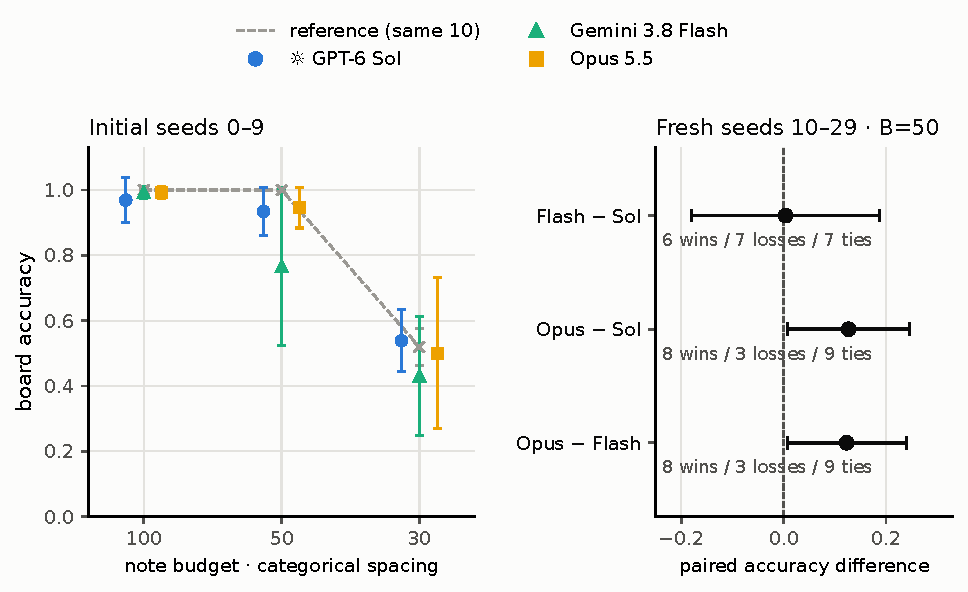
\includegraphics[width=\linewidth]{figures/relay_fig5_frontier.pdf}
\caption{Frontier-model board accuracy (fraction of keys correct) at tighter note budgets. Left: free-form means and across-seed 95\% $t$ intervals for three models and the reference on the same initial ten seeds. Budgets are categorically spaced. At $B{=}30$, GPT-6 Sol scores $\relayaddfreethirtysolsix$, slightly above the matched reference's $\relayfloorbthirtyshared$; equality is not established. Right: paired model differences on fresh seeds 10--29 at $B{=}50$, with 95\% $t$ intervals and sign-test win/loss/tie counts. No pairwise contrast survives the declared family correction (F15/F16).}
\label{fig:frontier}
\end{figure}

Neither the initial pairwise tests nor twenty fresh seeds at $B{=}50$ establish a ranking after correction. The 60-turn-cap condition also leaves the models near the ceiling, with guesses on turns $\relaylongfrontierguessmin$--$\relaylongfrontierguessmax$. It tests a larger available horizon with voluntary stopping. \Cref{app:frontier} gives the complete means, uncertainty, tie counts and family definitions. The pixel-channel results are reported separately in \Cref{app:pixel}.

\FloatBarrier
